\documentclass[a4paper]{article}
\usepackage[T1]{fontenc}
\usepackage[utf8]{inputenc}
\usepackage[italian]{babel}
\usepackage{lipsum}
\usepackage{verbatim}
\usepackage{graphicx}
\begin{document}
\section*{Relazione Smart Coffee Machine} 
\subsection*{Introduzione}
Lo scopo del progetto era quello di realizzare, tramite la piattaforma Arduino e la comunicazione seriale con una piattaforma realizzata in Java, un simulatore di una macchina del caffè intelligente, che con la rilevazione di movimento e distanza capisca quando accendersi, prepararsi per fare una caffè e tornare in modalità stand by.
\subsection*{Architettura e Progettazione Iniziale}
Siamo partiti con una progettazione orientata agli oggetti e che al suo interno includeva la creazione di più task, ognuno con un determinato compito e la possibilità di comunicare con gli altri attraverso delle variabili globali condivise.
\\ \\ \\
\textbf{Questi sono i seguenti task:}
\begin{itemize}
<<<<<<< Updated upstream
\item \textbf{MovementTask}:
=======
\item {MovementTask}:
Il MovementTask incapsula la logica per rilevare il movimento, cioè ciò che risveglia la macchina, esso contiene una classe PirSensor che implementa la logica di utilizzo del sensore PIR. Quando si crea una nuova istanza di esso bisogna dargli in ingresso il pin a cui il sensore(PIR) è agganciato. 
Quando il MovementTask viene inizializzato si richiama la sua funzione init() che prende in ingresso un periodo il quale specifica il quanto di tempo che intercorre tra due rilevamenti. 
Tale task viene eseguito quando il sistema si trova nello stato di \textbf{STAND BY}. Il MovementTask ad ogni tick del periodo assegna alla
variabile globale booleana movement che viene inizializzata nel setup l'input preso dal PIR. Se il sensore rileva movimento cioè, arriva in input un valore HIGH la variabile movement viene settata a true dal task sennò rimane a false come viene inizializzata da principio.  
Il task ha come stato iniziale \textbf{M0} che simula il fatto che non ci sia presenza, nel momento in cui viene rilevato un primo movimento passa a stato \textbf{M1}, per motivi di sicurezza si è deciso di gestire l'effettivo movimento solo dopo che il pir ha preso per due volte un valore HIGH, per questo il task passa da stato \textbf{M1} a stato \textbf{M2} dove viene settata la variabile movement. Sia da  \textbf{M1} che da \textbf{M2} si torna allo stato \textbf{M0} se il PIR non rileva più movimento. 
>>>>>>> Stashed changes

\begin{figure}[h!]
	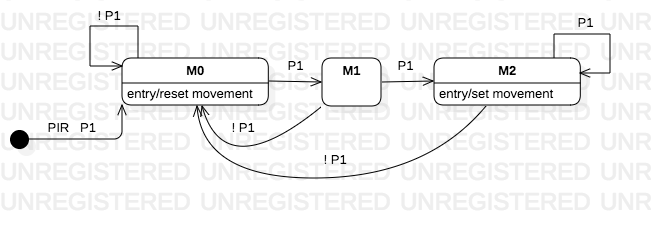
\includegraphics[scale = 0.60]{MovementTask.png}
	\caption{Diagramma a stati Movement Task}
\end{figure}

\newpage

<<<<<<< Updated upstream
\item \textbf{DistanceTask}:
=======
\item {DistanceTask}:
Il DistanceTask incapsula la logica per rilevare la distanza che intercorre tra la macchina e la persona. Si avvale di una classe Sonar che astrae il funzionamento del sensore per la rilevazione della distanza(SONAR). Come per il MovementTask anche esso ha bisogno di un periodo per gestire le rilevazioni sulla distanza, ad esso come al MovementTask è stato assegnato un periodo di 50ms. 
Il task viene eseguito quando il task principale cioè il \textbf{Main Task} si trova nello stato di \textbf{ON1} e \textbf{ON2} subito dopo che alla variabile movement è stata assegnata il valore true.
Ad ogni tick del periodo il task prende la distanza dal SONAR e la assegna alla variabile globale distance. Sia la variabile distance che movement vengono utilizzate per svegliare o addormentare il comportamento dei task. Per gestire il rilevamento corretto da parte del sonar si è deciso di utilizzare una media pesata dei valori, cioè i valori precedentemente rilevati avranno una priorità pari ad $\alpha$ invece il valore rilevato correntemente avrà priorità 1-$\alpha$ così da gestire gli sbalzi che il sensore ha in certi rilevamenti.   

>>>>>>> Stashed changes

\begin{figure}[h!]
	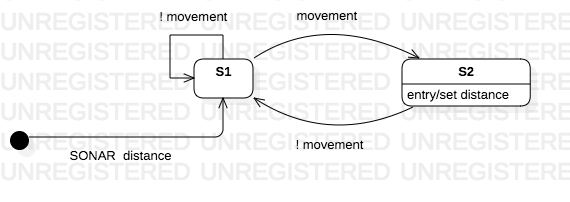
\includegraphics[scale = 0.60]{DistanceTask.png}
	\caption{Diagramma a stati Distance Task}
\end{figure}

\newpage


\item \textbf{Maintenance Task}:

Questo task gestisce lo scambio dei messaggi con la piattaforma realizzata su java attraverso la comunicazione seriale.

Tale task viene eseguito quando il sistema realizzato entra nello stato di MAINTENANCE. Tale variazione di stato viene espressa attraverso il set della variabile condivisa maintenance.
A questo punto il task controlla si mette in ascolto di messaggi in arrivo sulla seriale, in quanto attende il messaggio di ricarica che verrà inviato lato java, per effettuare la ricarica del caffè.

Tale messaggio contiene un stringa indicante il numero di caffè con cui ricaricare la macchina. Questo dato viene convertito in un intero e sommato alla variabile condivisa che tiene traccia dei caffè da poter fare.

Il messaggio ricevuto viene poi cancellato, in quanto Arduino non contiene il garbage collector, portando alla saturazione di memoria dopo pochi cicli di esecuzione.
E la variabile maintenance viene rosetta e si esce dallo stato di MAINTENANCE.

\begin{figure}[h!]
	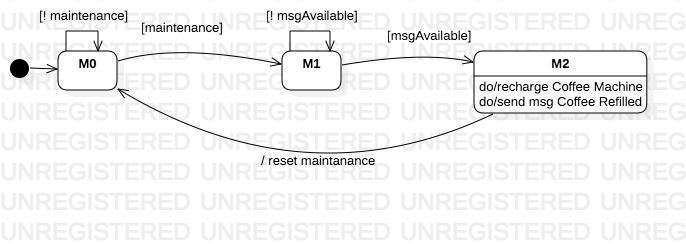
\includegraphics[scale = 0.50]{MaintenanceTask.png}
	\caption{Diagramma a stati Maintenance Task}
\end{figure}

\newpage

<<<<<<< Updated upstream
\item \textbf{MakeCoffee Task}:
Questo task gestisce la produzione di un caffè. Nel nostro sistema è emulata attraverso il lampeggiamento di tre led in sequenza, per la durata totale di 3 secondi.
Il tempo di accensione di ogni led viene tenuto memorizzato attraverso una variabile , che viene incrementata del periodo del task, ad ogni chiamata dello scheduler. 
In questo modo si riesce ad avere un periodo di esecuzione del task più basso, per essere responsivo, e una gestione dei led indipendente da esso.
Tale task entra in esecuzione quando viene impostata a true la variabile booleana condivisa makeCoffee, e viene impostata a false dal task stesso. In questo modo il task viene mandato in esecuzione da main task e dopo essere terminato, permette di capire al main task il cambiamento di stato. 
=======
>>>>>>> Stashed changes

\item {MakeCoffee Task}:

\begin{figure}[h!]
		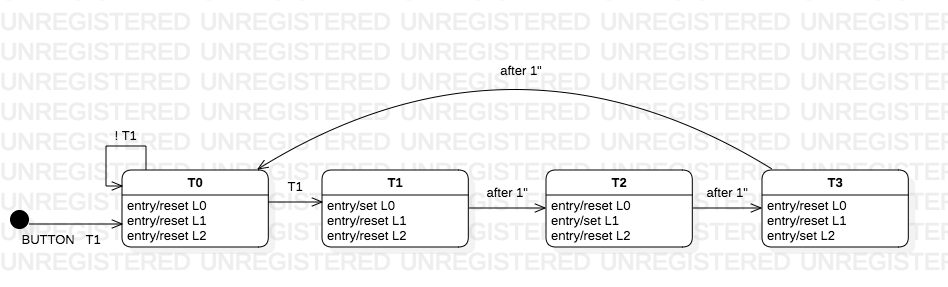
\includegraphics[scale = 0.40]{MakeCoffeeTask.png}
	\caption{Diagramma a stati Make Coffe Task}
\end{figure}

<<<<<<< Updated upstream
\item \textbf{Main Task}:



=======
\item {Main Task}:
Il Task principale di questo elaborato in grado di gestire la giusta sequenza di attivazione dei task è il Main Task, al quale è stato assegnato un periodo di 150.
Lo stato da cui il main task dovrà partire è quello di \textbf{STANDBY}, nel quale si attende la verifica del rilevamento di movimento data dal sensore pir nel suo task di riferimento, dal quale una volta accertata, si potrà passare allo stato di \textbf{ON}, nel frattempo il sistema dovrà entrare in uno stato di sleep dal quale risvegliarsi periodicamente ed effettuare il controllo di variabile.
Abbiamo deciso in fase di progettazione di dividere il funzionamento dello stato di \textbf{ON} in due stati: \textbf{ON1} e \textbf{ON2}, in quanto grazie a questa divisione diventa più facile gestire il lavoro a lui assegnato, in particolare ciò che deve fare il primo (\textbf{ON1}) è verificare che la variabile di movimento del Pir sia false (quindi ci sia assenza di movimento), nel qual caso bisognerà far partire un contatore e una volta raggiunto il tempo previsto faccia tornare la macchina allo stato di \textbf{StandBy} e inviare un messaggio di notifica sulla seriale a java, altro compito di questo stato è attendere che la distanza rilevata dal sonar diventi minore da DIST1 (quella richiesta), in tal caso il sistema dovrà eseguire una transizione di stato da \textbf{ON1} a \textbf{ON2} inizializzando un nuovo contatore a 0.
Entrati in \textbf{ON2} bisogna attendere che la variabile appena inizializzata raggiunga il tempo previsto DT1, se invece si ha un ritorno al valore della distanza rilevata dal sonar maggiore di DIST1, bisognerà tornare immediatamente a \textbf{ON1}, se invece viene raggiunto il valore di DT1 si effetua un nuovo cambio si stato verso \textbf{READY} e si invia un messaggio di notifica a java.
\textbf{READY}, come \textbf{ON}, si divide in 2 stati \textbf{READY1} e \textbf{READY2}. In \textbf{READY1} avremo la persistenza nell'attuale stato nel caso che la distanza rilevata dal sonar sia ancora un avolta inferiore a DIST1 e si avrà la possibilità di settare tramite il potenziometro il valore dello "zucchero" e inviarlo a java, nel caso che invece venga premuto il bottone T1 si dovrà inviare la notifica a java ed effetuare un cambio di stato a \textbf{MAKECOFFEE} che in questo task avrà soltato il compito di settare la variabile makecoffe = a true, cosi facendo si da la possibilità al Task \textbf{MAKECOFFEE} di essere eseguito una volta richiamato dallo Scheduler, se invece la distanza rilevata diventa maggiore di DIST1 si inizializza un nuovo contatore e si passa allo stato di \textbf{READY2}, il quale avrà il compito di aspettare che il contatore arrivi al tempo previsto DT2 e in tal caso si avrà un ritorno allo stato di \textbf{ON1}, mentre se invece la distanza torna ad essere inferiore a DIST1 un ritorno a \textbf{READY1}.
\textbf{MAKECOFFEE} ha il compito di inviare tramite seriale un messeggio a java per far sapere che ci si trova nello stato attuale, incrementare la variabile numCoffee, segnalatrice del numero di caffè già generati, e nel caso siano finite "le ricariche" (quindi si raggiunga un certo valore) si abbia un cambio di stato a \textbf{MAINTAINCE}, l'invio di un messaggio a java del cambio effettuato e l'assegnamento della variabile maintaince a true in modo da poter eseguire il suo task associato, comunque una volta che il task di \textbf{MAKECOFFEE} viene eseguito (il quale dovrà rispettare un determinato periodo) si torna allo stato \textbf{READY1}.
Nello stato \textbf{MAINTAINCE} si dovrà tornare allo stato di \textbf{STANDBY} una volta eseguito il suo rispettivo task.

\begin{figure}[h!]
	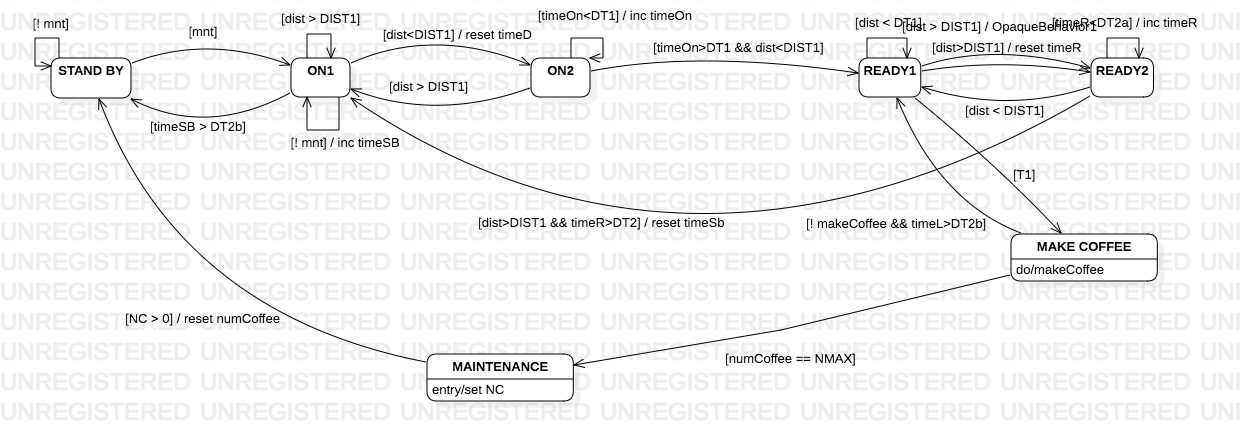
\includegraphics[scale = 0.30]{MainTask.png}
	\caption{Diagramma a stati Main Task}
\end{figure}
>>>>>>> Stashed changes




\end{itemize}
\subsection*{Progettazione specifica}
Durante la fase di design del progetto un pò più approfondita abbiamo deciso di considerare il main task,  il task principale che gestendo gli stati del sistema, avrebbe fatto da controllore per far eseguire gli altri task nel momento opportuno. In quanto gli altri task possono essere divisi in due tipologie:
\begin{itemize}
\item {Task di rilevazione }:
Questi task assegnano il valore letto dai sensori alle corrispettive variabili condivise, in modo da permettere al main task di avere i dati dei sensori sempre aggiornati, ma senza doversene occupare lui direttamente.


\item {Task di esecuzione }:
In modo differente, questi task vengono "avviati" dal main task ed eseguono delle routine come il lampeggiamento dei led e la comunicazione con la piattaforma in Java.
Spiegandoli in modo più accurato, questi task vengono eseguiti dallo scheduler in continuazione come gli altri task e con stessa priorità, ma allora interno hanno un semplicissimo controllo sulla variabile condivisa rispettiva e nel caso in cui sia a false, il task non esegue niente. Altrimenti viene eseguita la routine specificata.

\end{itemize}

Durante questa fase, cia siamo imbattuti nella decisione di dove eseguire la modalità di risparmio energetico nello stato STAND BY. Inizialmente avevamo pensato una soluzione in cui tale operazione veniva gestita da un task a se stante, ma dopo varie considerazione abbiamo deciso per l'inserimento della sleep mode all'interno del main task, in quanto essendo il task principale era giusto che una funzionalità importante come questa fosse gestita al suo interno. 
Per la sua implementazione successiva c'erano due possibilità:  l'assegnamento di un interrupt al sensor PIR, che risvegliasse il micro controllore quando veniva rilevato un movimento. Una sleep mode ciclica che si risvegliasse periodicamente con il timer di esecuzione dello scheduler.
Fra le due soluziono abbiamo optato per la seconda in quanto abbiamo voluto mantenere il sistema basato su macchina totalemte sincrona, evitando qualsiasi elemento asincrono.



\newpage
\null
\vfill
Enrico Gnagnarella, Anis Lico, Tommaso Ghini
\clearpage

\end{document}